% !TeX spellcheck = en_GB
\chapter{Main Objectives}
\begin{comment}
Generally valid: leave it here for us.
\todo[inline]{Charlie: we have to be careful with our terminology across different sections}
\todo[inline]{Charlie: each section if applicable should explain why? who? what? where? how?}

\end{comment}

\section{Overview} 
The goal of this project is to design, implement and provide a guidance platform for the developing country Afghanistan. 
Taking the circumstances in such a developing country in account, the platform should provide the users of IT-systems with the knowledge to assure the sustainability of IT-systems in their countries. 
Besides providing general information on IT-systems, the platform should provide, similar to the “BSI Grundschutzkatalog”, information aiming to localize and solve problems that may occur in the IT-systems as a result of a human error, technical failure or a catastrophe etc. 
\\
\begin{figure}[h] 
    \centering
    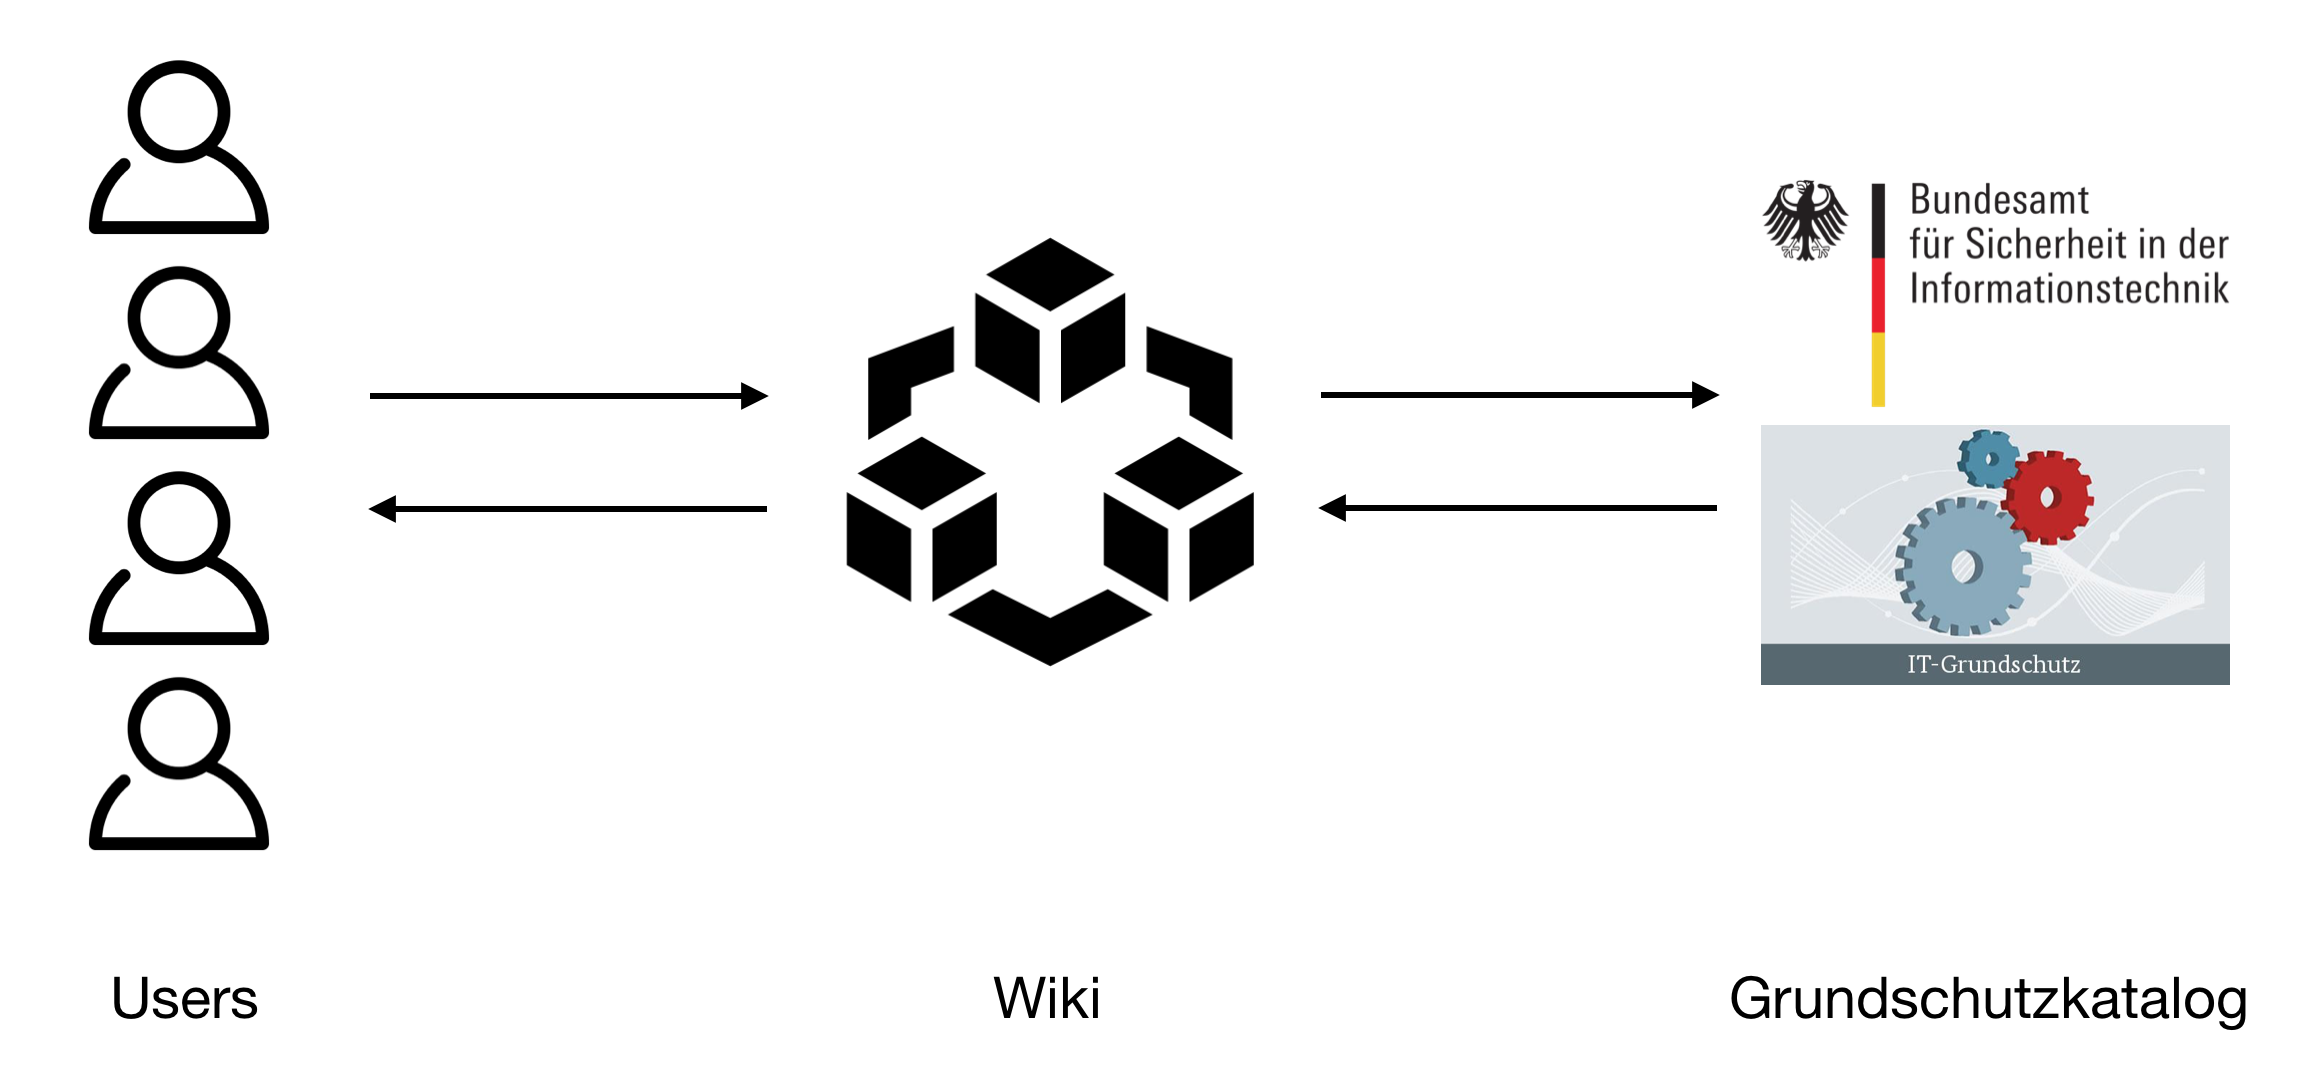
\includegraphics[scale=0.3]{Pictures/ConceptSketch}
    \caption{Abstract System Design}
\end{figure} 


\section{Wiki} 
Considering the limited availability of IT-specialists in most of the developing countries, and after reviewing the possible ways to design and provide the platform, our team considers it convenient to create an open platform on which people can collaboratively add, edit, delete or archive content, similar to Wikipedia. 
This should allow the platform to constantly grow and stay relevant to current circumstances. 
The user created content beyond the BSI catalogue could make remarks about national peculiarities that do not play a role in Germany, aid further understanding or offer updates on more recent developments.
However, this should not mean that everyone can simply write any potentially false content for everybody to read. 
To assure that we have to set rules and access permission levels (see section~\ref{user_types}). 
Concretely the wiki should have the following parts:
\begin{itemize}
    \item News
    \item BSI catalogue
    \item Articles
    \item Archive
\end{itemize}
which will be further explained in the next subsections.
\begin{tcolorbox}[breakable,colback=red!12,colframe=red!40!black,title=UPDATE 15/11/2017]
In general, it should be possible to link from any page in the wiki to any other page (see Secondary Objectives~\ref{2nd_bsi_link} for special requirements regarding the BSI catalogue). 
General wiki behaviour as found on i.e. wikipedia.org applies:
\begin{itemize}
    \item each word on any page can only link to one other page at a time,
    \item users who collaboratively work on the same wiki page can edit or delete each others text or links,
\begin{tcolorbox}[breakable,colback=red!14,colframe=red!40!black,title=UPDATE 19/11/2017]
    \item each page should have a history page where different versions of the page over time can be checked,
    \item it is possible to retrieve a list of all users who ever worked on a given page in the wiki
\end{tcolorbox}
        .
\end{itemize}
\end{tcolorbox}


\subsection{Links}
\begin{tcolorbox}[breakable,colback=red!14,colframe=red!40!black,title=UPDATE 19/11/2017]
Links are represented in two ways which slightly differ in the domains of news, articles and catalogue.
A link can be:
\begin{enumerate}
    \item \ldots a text link where the linked page directly comments on a word or phrase.
                \begin{comment}
        \begin{enumerate}
            \item On article and news pages these are word links which means a single word is highlighted and represents the link.

            \item On BSI catalogue pages a link belongs to a word but is displayed at the right of the text.
                The word is not highlighted, instead there is a small but obvious mark next to the line of the text.
                This mark could be a small uni-coloured area or a symbol and each line that has a link has a mark next to it.
                When guests hover with their mouse over the mark a small pop-up should appear informing the guests which word of the text line links to which other page.
                The other page should be given by its title not URL.
                If a text line contains several links they are aggregated in a single mark.
                This is thought to improve the readability of the BSI catalogue and to underline its quality as an official source as opposed to user created wiki content.
        \end{enumerate}
                \end{comment}
    \item \ldots a bottom page link in section called 'See also' after the page content that is commenting on the wider scope of the whole page. 
        News have no bottom page links.
        .
\end{enumerate}
\end{tcolorbox}

\subsection{News}
News are written by users but have to be approved by mods.
If a mod approves a news article it is automatically published on the home page.
The mod can decide to make a news article an important news article.

\begin{tcolorbox}[breakable,colback=red!14,colframe=red!40!black,title=UPDATE 30/11/2017]
News should be implemented in the same best-practice way of Wikipedia.
One article for each month, including subsections for each day and links to previous months or years.
Here is an example:  \url{https://de.wikipedia.org/wiki/November_2017}.
However, news were categorized as lower priority feature by the programming group. 
\end{tcolorbox}


\subsection{BSI Catalogue}
\label{BSIc}
The BSI catalogue spans over 5000 pages which makes browsing, or even searching a specific information, a difficult task for beginners. 
Converting such a big text volume into wiki content by hand would be an extended task. 
Accordingly, a parser is needed. 
This parser will crawl and analyse the BSI Grundschutzkatalog website and create and sort the content automatically. 
The BSI catalogue is the most restrictive part in the wiki and should only be modifiable by administrators.
\begin{tcolorbox}[breakable,colback=red!12,colframe=red!40!black,title=UPDATE 15/11/2017]
    Should users find any mistakes on the pages of the BSI, i.e. something is translated badly, the users have to inform an administrator who has to correct the text in question.
\end{tcolorbox}
\bigskip

While browsing any page of the BSI catalogue a tree view of the catalogue should be displayed at the side.
\bigskip

\begin{tcolorbox}[breakable,colback=red!10,colframe=red!40!black,title=UPDATE 13/11/2017]
The tree view adopts the structure as also found in pdf versions of the BSI catalogue. 
See Appendix~\ref{appendix_bsi}.\\
The tree view should not automatically expand or collapse itself without direct guest manipulation.
This means for instance, that when a guest, clicks on the link of a threat on a building block page that the tree view does not expand to show this threat.
Merely the highlighted row in the tree view changes to the new item.
If the item is hidden in a collapsed level the highlighted row should change colour.
\\
BSI pages which show building blocks should be displayed slightly modified from their appearance in the catalogue.
Instead of listing threats and measures seperately in lists, it should be obvious only after a quick glance which measures corresponds to which threats.
For this, cross-reference tables provided by the BSI should be used.
These tables clearly assign each threat its measures.
Thus, those pages show firstly the related text to the building block.
Then a dropdown menu which allows the guest to sort the linked threats and measures by either threats or measures.
Lastly, a tree view where the first level are layers, the second level the category by which the tree is sorted and the third level the other category.
See Appendix~\ref{appendix_bsi} for examples.
\end{tcolorbox}


\subsection{Archive} 
\label{archive}
The website should always present up-to-date information for interested guests.
Sometimes though a person might be interested in information on older systems which are not covered anymore in the most recent version of the BSI catalogue but in older versions.
Those older versions and ideally their related wiki content should be available in the archive. 
On the matter of the related content see section~\ref{archive_relcon}.

For example: if users are looking for an information on a no longer supported operating system and there are none in the wiki regarding this problem, the user could find older approaches in the archive. 

\begin{tcolorbox}[breakable,colback=red!14,colframe=red!40!black,title=UPDATE 19/11/2017]
Content in the archive can not be edited.
It stays as it is since the moment it is moved to the archive.
\end{tcolorbox}


\subsection{Updating the BSI Catalogue}
\begin{tcolorbox}[breakable,colback=red!14,colframe=red!40!black,title=UPDATE 19/11/2017]
Updating the BSI catalogue to a newer version happens in three phases:
\begin{enumerate}
    \item before the update: an admininistrator decides to update and performs the necessary action,
    \item during the update: re-linking of pages,
    \item after the update: the website is up-to-date again and old content is in the archive 
\end{enumerate}

About 1., the update can only be kicked-off by an administrator.
The necessary action should be as simple as possible. 
\begin{comment}
Ideally the admin just has to click a button.
\end{comment}
\bigskip

About 2., during this phase the website will be in a hybrid state.
While the current catalogue is still available via 'Browse BSI' in the Top Section (see section~\ref{top_section}) the new catalogue will be advertised in the news section on the landing page.
It should stick to the top of the news list and be marked as important news.
With the end of phase 1 of the update users get a notification that articles they worked on in the past have to be re-linked.
This means all the articles which are linked to the BSI catalogue and which therefore are to be considered outdated until proven otherwise by a user.
At the same time there should be a page in the forum or wiki visable to all users that lists all the articles in question which have not been re-linked yet.
With the end of phase 2 all pages which link to the catalogue that gets archived are moved to the archive as well.
Pages which were re-linked to the new catalogue are copied versions.
This is necessary because articles in the wiki could be edited to reflect real world changes. 
Those edits then still apply to the new BSI catalogue but might not apply for older versions.
Therefore, for every BSI catalogue version since the article was written and as long as it got re-linked the archive contains the same pages again which are not identical ones.
\medskip

The news section on the landing page should also link to a change log page that informs about dropped, inserted and altered catalogue parts. 
\bigskip

About 3., after a certain time - i.e. 30 days - the admin might choose to complete the process.
The catalogue which up to now was accessible via 'Browse BSI' gets pushed into the archive including its wiki articles.
The new catalogue gets is linked to the top section and the important news on the landing page can slowly drop down as other news come in.
\end{tcolorbox}


\subsection{User Types} 
\label{user_types}

First of all, the platform will need one or multiple administrators (admins) who will update the platform from a technical perspective and ensure that policies are being respected. 
However, building a wiki-like platform about IT-Security for developing countries comes also with the big responsibility of the content it will provide. 
If everybody could publish and/or modify content without checks or labels for flaws, or malicious informations, it would present a major security risk for any layman reading it. 
Admins will have enough workload so we need another team of volunteers, like moderators (mods), who will check content and remove, modify or label it as unsafe if necessary. 
Moderators will be appointed by admins and will be responsible for policy enforcement for specific topics. 
Further, users who would like to publish and/or modify content will need to register to the platform and be logged in. 
All other users who are not logged in will be considered as guests and will only be able to read content. 
The following section will discuss the different user roles and their functions. 
%We decided to create four types of users with different user rights. 
This is illustrated in the appendix by the use case diagrams. 
\bigskip

\textbf{Guest}, the guests have the possibility to browse and search in the archive and also in the wiki, which includes the BSI catalogue. The search can be refined with several options (more information about the search in the text search section~\ref{search_function}) 
If guests are not sure how to find their problems they can use the wizard (more information in the wizard section~\ref{wizard}). 
The wiki contains news from different topics which guests can check out.
\bigskip

\textbf{User}, every registered user (registed by email address and a password) can write articles in the wiki and change them with the functions: create content and edit content. 
Created content can be linked in a certain part of the BSI catalogue. 
If the BSI catalogue updates, users who have linked content get a notification to transfer this link to the new BSI catalogue or to archive the linked wiki article with it.
They can also edit their profile. 
After a User has logged in, he can still use the functions of a guest.
\bigskip

\textbf{Moderator} (mod), mods are managing the content published by the users.
Managing or Moderating content means to delete wrong or inappropriate content or make checked content recognizable for guests that the content is verified.  
Mods manage the news which means they can show certain news on the home page to get more attention or delete/change incorrect news. 
Mods are also responsible, if necessary, to ban users. 
Mods can use all functions users can use.
\bigskip

\textbf{Administrator} (admin), the admin sets or changes permissions like banning users, assign topics and manage news.
One of the most important tasks of the admin is to update the BSI catalogue as soon as a new one is available and to move the old one to the archive.  There should be two admins for the website in case one is non-available.
The admin can use all functions mods can use. 
\bigskip

The table \ref{fig:usertypes} shows the rights of each user.

\begin{figure}[h]
    \centering
    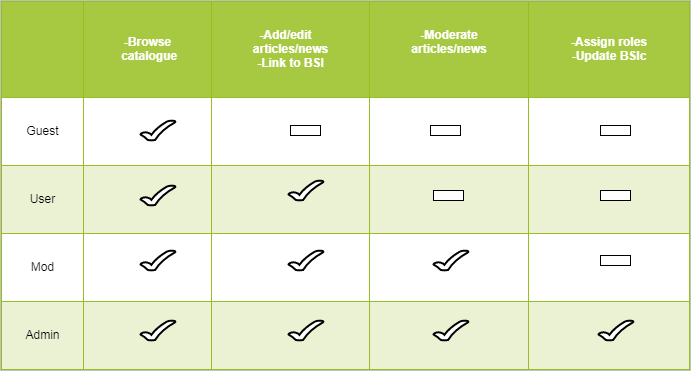
\includegraphics[width=0.9\textwidth]{Pictures/user_types}
    \label{fig:usertypes}
    \caption{user rights table}
\end{figure}

\section{Text Search}
\label{search_function}
A text search function allows users of the platform to make a free text search request and browse the results containing the key-words. 
Users should also have the opportunity to narrow down their search request by selecting a specific domain in which they would like to find results:
\begin{itemize}
\item "All": counts as every domain
\item "News": domain where news are published
\item "Module": modules of the BSI Grundschutzkatalog
\item "Threats": threats of the BSI Grundschtzkatalog
\item "Measures": measures of the BSI Grundschutzkatalog
\item "Archive": archived content (no longer visible in the wiki)
\end{itemize}
 
Choices should be available as a dropdown list.
\bigskip

The search field should be well placed on the home page. 
The system should have a function "Back to the search results". 
The search function should have fault tolerance, as well as the ability to deal with synonyms. 
Fault tolerance means that the user will get the result even if he misspells a word or if he uses singular or plural. 
While a non-fault-tolerant search will let the visitor go nowhere, the system should nevertheless display the appropriate results.
In addition, search functions which also master synonyms, do even more. 
For example, the system should derive results from the search input "laptop" in which the word "notebook" appears and for this purpose access an extensive database of words of the same meaning. 
The automatic completion of search terms is very welcome.
  

\section{Wizard}
\label{wizard}
Beginners who are not familiar with the terminology may have a hard time finding solutions to problems they encounter. 
To help them, we would like to implement a wizard, which will ask them a set of yes/no questions to filter out what problems they could have, similar to the game Akinator\footnote{\url{http://en.akinator.com}}. 
 
\section{Home Page}
The home page is the entry point to the different services offered by the website. 
As such its design should provide a clear overview of and a dead on target guidance to all available functions for users of all levels of experience.
Firstly, the home page also displays the always present top section (see section~\ref{top_section}) but no side bar to use the full available space for the sections defined below and in order to not overwhelm the user with two detailed lists of items.
Directly below the top section is a distinguished area for time-critical news which inform of widespread threats or important updates.
Those are important to all users and should therefore be on top.
In times of no imminent danger time-critical news might not be displayed but instead a few of the most recent regular news which are part of the wiki.
The third area in a vertical sense is a wide and inviting search bar that allows experienced users the quick access to the BSI catalogue and other parts. 
Should a user not know what to search he can browse the BSI catalogue following a link in the top section (see section~\ref{top_section}).
The search offers the full functionality as described in section~\ref{search_function}.
As a last section before the always present bottom section is an overview of introductory tutorials on how to implement the guidelines of the BSI catalogue while developing, building and maintaining a basic IT system.
Equally visible as the tutorials should be the offer to use the wizard to help and find security gaps and other system flaws.
Both the tutorials and the wizard are aimed at users of no or little knowledge or overview of the BSI catalogue.
For detailed explanations of the wizard see section~\ref{wizard}.
The bottom section shows links to items as contact, legal notice, possibly FAQ and copyright.

\begin{figure}[h]
    \centering
    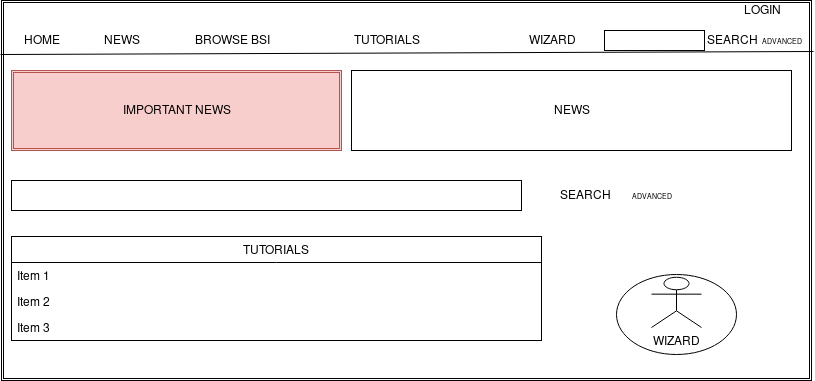
\includegraphics[width=0.9\textwidth]{Pictures/frontpage_mockup}
    \caption{Schematic Home Page Design}
\end{figure}
 
\section{Top Section}  
\label{top_section}

The top section is an always present area at the top of each subpage that connects the different services and allows for quick access.
It should feature the following items whose order and wording might be changed appropriately:
\begin{itemize}
    \item Home Page
    \item News
    \item Browse the BSI catalogue
    \item Tutorials
    \item Wizard
    \item Search
    \item Login  
        . 
\end{itemize}


%\section{Tutorials}
%\label{tutorials}

%Tutorials should call unexperienced users' attention to the most important points in the BSI catalogue when developing, building or maintaining an IT infrastructure.
%They could briefly explain mayor points of the BSI catalogue and indicate next steps.
%The simplest tutorial could simply introduce the usage and goal of the website and its subservices.
%The tutorials are not meant to be a rewrite - i.e. the BSI catalogue for dummies - but thought of as a quick overview and guiding introduction into the matter.
%They are part of the wiki and as such created and maintained by content manager and linked by mods.
%\todo[inline]{to remove?}
